% File:		curve.tex
% Author:	See Below
% Date:	        See Below
%
% The authors have placed this file in the public domain;
% they make no warranty and accept no liability for this file.

\documentclass[12pt]{article}
\usepackage{times}
\usepackage{color}
\usepackage[usenames]{xcolor}
\usepackage{scalefnt}
\usepackage{tikz}
\usepackage{wrapfig}
\usetikzlibrary{arrows}
\begin{document}
\newcommand{\header}[1]{\underline{\bf #1}}
\newcommand{\file}[1]{{\bf #1}}
\newcommand{\blankpage}{\newpage\vspace*{3.5in}%
    \centerline{\Large This Page is Intentionally Left Blank}}
\setlength{\parindent}{0.0in}
\setlength{\parskip}{1ex}
\newcommand{\key}[1]{{\bf #1}}
\newcommand{\TT}[1]{{\tt \bfseries #1}}
\newcommand{\EOL}{\penalty \exhyphenpenalty}
\newtheorem{definition}{Definition}[section]
\newtheorem{lemma}[definition]{Lemma}
\newtheorem{corollary}[definition]{Corollary}
\newtheorem{theorem}[definition]{Theorem}
\newtheorem{algorithm}[definition]{Algorithm}
\newenvironment{indpar}[1]%
    {\begin{list}{}{\setlength{\leftmargin}{#1}}\item[]}%
    {\end{list}}

\begin{center}
{\Large \bf Two Dimensional Analytic Curve Calculator}

\begin{tabular}{ll}
Author:	      & Robert L.~Walton $<$walton@acm.org$>$ \\
Date:         & Sun Jul 18 14:48:01 EDT 2021
\end{tabular}
\\[2ex]
\begin{tabular}{p{5in}}
The author(s) have placed this document and associated problems
in the public domain;
they make no warranty and accept no liability for this document
or associated problems.
\end{tabular}

\end{center}

\medskip

\section{Overview}
This document describes a group of 2-dimensional geometry problems
based on analytic curves, e.g., circles, ellipses, parabolas.
The problems are embedded in an extension of the
vec-2d problem calculator for ease of
testing.

For theory we assume familiarity with the vec-2d document, and for
code we assume that code for a vec-2d calculator is available to extend.



\section{Circle, Line, and Point}
In this section we investigate the following questions:
\begin{enumerate}
\item What is the distance between a point and a circle (viewed as
a curving line and \underline{not} an area)?
Is the point on the circle?
\item Where do the lines tangent to a circle that pass through
an external point contact the
circle?
\item Does an infinite line intersect a circle?  Is it
tangent to the circle?  Where does it intersect?
\item What is the distance between a finite line segment and
a circle?  If zero, where are the intersections?  If not zero,
where is the point on the finite line segment that is closest to the
circle.
\end{enumerate}

Suppose we have a point {\tt p} and a circle with center {\tt c}
and radius {\tt r>0}.  Then the distance from {\tt p} to the circle
is the absolute value of {\tt ||p-c|| - r},
where we view the circle as a closed line
and \underline{not} as an area.

To precisely test whether {\tt p} is outside, on, or inside the
circle, assuming that input coordinates and {\tt r} have at most
{\tt d} decimal places, we can use the equations:
\begin{center}
\begin{tabular}{l@{~~~~~}l}
\tt r$^2$ < (p-c)*(p-c):(2d) & outside the circle \\
\tt (p-c)*(p-c) == r$^2$:(2d) & on the circle \\
\tt (p-c)*(p-c) < r$^2$:(2d) & inside the circle \\
\end{tabular}
\end{center}


\begin{minipage}{\textwidth}\raggedright
\label{TANGENT-PICTURE}
\begin{wrapfigure}{r}{0.3\textwidth}
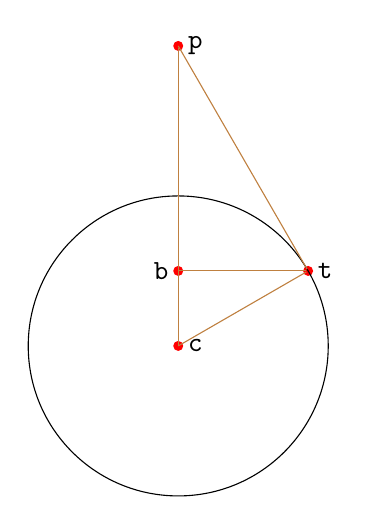
\begin{tikzpicture}[x=0.25in,y=0.25in]
\begin{scope}[>=triangle 45,shorten >=0.01in]

    \fill[red] (0,6.0) circle(0.1);
    \draw[black] (0,6.0) node[right]{\tt p};
    \fill[red] (0,0) circle(0.1);
    \draw[black] (0,0) node[right]{\tt c};
    \fill[red] (0,1.5) circle(0.1);
    \draw[black] (0,1.5) node[left]{\tt b};
    \fill[red] (2.598076,1.5) circle(0.1);
    \draw[black] (2.598076,1.5) node[right]{\tt t};


    \draw[black] (0,0) circle(3.0);
    \draw[brown] (0,0) -- (0,6.0);
    \draw[brown] (0,1.5) -- (2.598076,1.5);
    \draw[brown] (0,6.0) -- (2.598076,1.5);
    \draw[brown] (0,0) -- (2.598076,1.5);


\end{scope}
\end{tikzpicture}
\end{wrapfigure}
Now suppose that {\tt p} is outside the circle and we want to find
a point {\tt t} on the circle such that {\tt pt} is tangent to the
circle.  See the picture. \\
~ \\
\label{FINDING-TANGENT-POINT}
We define {\tt b} to be the point on {\tt pc} such that
{\tt tbp} is a right angle.  Then we have: \\
\hspace*{0.2in}\begin{tabular}{@{}l} \\
    {\tt ptc} is a right angle \\
    {\tt ||p-c||} is known \\
    {\tt ||t-c||=r} \\
    angle {\tt pct} equals angle {\tt tcb} \\
    triangles {\tt ptc} and {\tt tbc} are congruent \\
    so {\tt \small ||b-c||/||t-c|| = ||t-c||/||p-c||} \\
    so {\tt \small ||b-c|| = r$^2$/||p-c|| = r$^2$/L} \\
    where {\tt L = ||p-c||} \\
    \end{tabular}
\end{minipage} \\
\hspace*{0.2in}\begin{tabular}{@{}l}
    and using \\
    {\tt ||b-t|| = $\sqrt{{\tt r}^2 - {\tt ||b-c||}^2}$ =
                   (r/L)*$\sqrt{{\tt L}^2 - {\tt r}^2}$} \\
    we can compute both {\tt ||b-c||} and {\tt ||b-t||}; \\
    then if we define {\tt u = <p-c>} we have \\
    {\tt b = c + ||b-c||*u = c + (r$^2$/L$^2$)*(p-c)} \\
    {\tt t \begin{tabular}[t]{@{}l}
         = b $\pm$ ||b-t||*(u\textasciicircum 90) \\
         = b $\pm$ (r/L$^2$)*$\sqrt{{\tt L}^2 - {\tt r}^2}$%
	                    *((p-c)\textasciicircum 90) \\
	   \end{tabular}} \\
    \end{tabular}

The reason for the $\pm$ is that we actually have two possible
values for {\tt t}, one on either side of the line {\tt pc}.

Since we are using a computer, the inputs {\tt r} and the coordinates
of {\tt p} and {\tt c} must be rational.  Then
the coordinates of {\tt b} are rational
with denominator containing {\tt (p-c)*(p-c)}.  However, the
coordinates of {\tt t} are irrational in general, due to
$\sqrt{\tt (p-c)*(p-c) - r*r}$ being a factor while other factors are rational.
For example, if {\tt ||p-c|| = 3} and {\tt r = 1}, then
$\sqrt{\tt 3*3 - 1*1} = \sqrt{\tt 8} = {\tt 2*}\sqrt{\tt 2}$
is irrational.  However note that the coordinates of {\tt t}
will be rational if
{\tt (r,||p-t||,||p-c||) = (r,$\sqrt{{\tt L}^2 - {\tt r}^2}$,L)}
is a rational number times a pythagorean triple.

Now let {\tt p} and {\tt q} be points on an infinite line {\tt pq}
and let {\tt c} be a circle of radius {\tt r}.  Does {\tt pq} intersect
the circle, and is it tangent?

If {\tt pq} is tangent, the point {\tt t} where it intersects the
circle is also the point on the line closest to {\tt c}.  By
the argument presented in Line and Point of the vec-2d problems,
if {\tt p}, {\tt q}, and {\tt c} all have rational coordinates, then
{\tt t} will have rational coordinates, but by the argument immediately
above, it will usually have irrational coordinates.  From this
we conclude that {\tt pq} is usually not tangent to the circle
if {\tt p}, {\tt q}, and {\tt c} all have rational coordinates and
{\tt r} is a rational number.

\bigskip

\begin{minipage}{\textwidth}\raggedright
\label{INTERSECTION-PICTURE}
\begin{wrapfigure}{r}{0.5\textwidth}
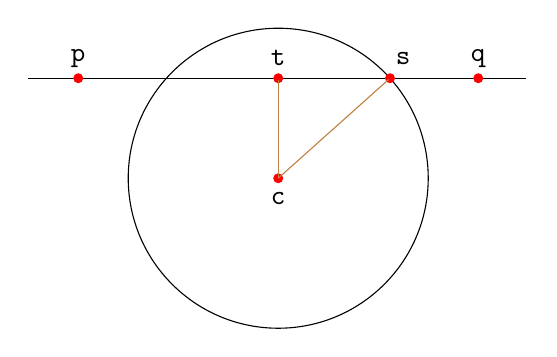
\begin{tikzpicture}[x=0.25in,y=0.25in]
\begin{scope}[>=triangle 45,shorten >=0.01in]

    \draw[black] (0,0) circle(3.0);
    \fill[red] (0,0.0) circle(0.1);
    \draw[black] (0,-0.4) node{\tt c};

    \draw[black] (-5.0,2.0) -- (+5.0,2.0);
    \fill[red] (-4.0,2.0) circle(0.1);
    \fill[red] (+4.0,2.0) circle(0.1);
    \draw[black] (-4.0,2.4) node{\tt p};
    \draw[black] (+4.0,2.4) node{\tt q};

    \fill[red] (0,2.0) circle(0.1);
    \draw[black] (0,2.4) node{\tt t};

    \draw[brown] (0,0) -- (0.0,2.0);

    \fill[red] (2.236068,2.0) circle(0.1);
    \draw[black] (2.5,2.4) node{\tt s};
    \draw[brown] (0,0) -- (2.236068,2.0);

\end{scope}
\end{tikzpicture}
\end{wrapfigure}
So let us just assume for the moment that the line intersects
the circle, and locate the points of intersection (see picture).
By the Line and Point section of the vec-2d problems,
we can find the point {\tt t} on the line that is closest to
{\tt c}, and find the distance {\tt ||t-c||}.  Then the line {\tt tc} is
perpendicular to {\tt pq}, as if it were not, we could
reduce {\tt ||t-c||} by sliding {\tt t} along the line {\tt pq}.
If {\tt s} is an intersection point of {\tt pq} and the circle, we have: \\
\hspace*{0.2in}\begin{tabular}{@{}l}
    {\tt ||s-c||$^2$ = r$^2$ = ||t-c||$^2$ + ||t-s||$^2$} \\
    so {\tt ||t-s|| = $\sqrt{{\tt r}^2 - {\tt ||t-c||}^2}$} \\
    and if we define {\tt u = <q-p>} we have \\
    {\tt s = t $\pm$ ||t-s||*u} \\
    \end{tabular}
\end{minipage}

The reason for the $\pm$ is that we actually have two possible
values for {\tt s}, one on either side of the line {\tt tc}.

The distance {\tt ||t-s||} goes to zero as {\tt ||t-c||} approaches
{\tt r}, and cannot be computed if {\tt ||t-c|| > r}, in which case
the line is completely outside the circle and does not intersect the
circle.

We end this section by examining the case of a \underline{finite}
line {\tt pq} and a circle with center {\tt c} and radius {\tt r}.
Find the point {\tt t} on the infinite line {\tt pq} closest to
{\tt c}, and the points {\tt s} that where the infinite line intersects
the circle, if they exist.
Then use the {\tt (q-p)*} product to establish coordinates on the
infinite line: \\
\centerline{\tt (q-p)*p ~~~ (q-p)*q ~~~ (q-p)*t ~~~ (q-p)*s}
Since {\tt (q-p)*p~<~(q-p)*q},
{\tt t} is in the finite line {\tt pq} if and only if \\
\centerline{\tt (q-p)*p $\leq$ (q-p)*t $\leq$ (q-p)*q}
Similarly we can find out if an intersection point is on the finite
line.

So what points on the finite line {\tt pq} are closest to the circle?
If finite {\tt pq} intersects the circle these are the intersection points.
Otherwise there are two cases: {\tt pq} is outside the circle and
{\tt pq} is inside the circle.

To make further progress, we are \underline{not} going to use the fact that the
circle is a circle.
Instead we will use the fact that the circle viewed
as an area is a closed convex set, and the circle viewed as an arc
is the boundary of such a set.  This allows us to prove our results
for closed convex sets, and apply the results to circles, ellipses,
rectangles, and convex polygons.

\begin{definition}
The \key{boundary} of a set $S$ of the points in the plane
(i.e., $S\subset\mathcal{R}^2$) is the
set of points $p$ such that every circle with
center $p$ contains inside it a point in $S$ and another point not in $S$.

A set $S$ of points in the plane is \key{closed} if every point
of the boundary of $S$ is in $S$.

A set $S$ of points in a plane is a \key{bounded set} if and only if
there is a circle that includes $S$.
\end{definition}

We need $S$ to be closed in order to use the notion of
closest point.

\begin{lemma}\label{MINIMUM-DISTANCE}
Let $S_1$ and $S_2$ be close sets one of which is bounded.
Then there are points
$p_1\in S_1$ and $p_2\in S_2$ such that $||p_1-p_2||$ is as
small as possible (i.e., for every $q_1\in S_1$ and $q_2\in S_2$,
$||q_1-q_2||\ge||p_1-p_2||$).
\end{lemma}

We will \underline{not} give the proof of this,
which involves the mathematics of compact
sets (i.e., uses the fact that a closed bounded set is compact).

Some facts about boundaries are:
\begin{enumerate}
\item The boundary of a set $S$ is also the boundary of the
complement $\mathcal{R}^2-S$ of $S$.
\item The boundary $B$ of a set $S$ is itself closed
(i.e., $B$ is a closed set).
\end{enumerate}
\begin{indpar}{0.3in}
Proof:  The first fact is easy.  For the second fact, let
$p$ be a point in the
boundary of $B$.  Then every open circle centered at $p$
contains inside it a point $q$ in $B$ and a smaller circle
centered at $q$ that is inside the first circle, and this
smaller circule contains
inside it a point in $S$ and a point not in $S$.  So $p$ is in $B$.
\end{indpar}


Another important fact about closed sets and their boundaries is:

\begin{lemma}\label{BOUNDARY-CROSSING}
If $S$ is a closed set, $p$ is a point in $S$, and $q$ is a point
outside of $S$, then the finite line $pq$ contains a point on the
boundary of $S$.
\end{lemma}
\begin{indpar}{0.2in}
Proof: Consider the points $r=p+\alpha*(q-p)$ for $0\le\alpha\le 1$,
that is, the points $r$ on the finite line $pq$.
All circles with center $p$ contain a point of $S$ as $p$ is in $S$.
All sufficiently small circles with center $q$ contain only points
outside of $S$, as $q$ is outside of $S$ and not on the boundary of $S$
(which is a subset of $S$).  Let $\alpha'$ be the smallest number such
that $r=p+\alpha*(q-p)$ is outside $S$ for all $\alpha>\alpha'$ and
let $r_0=p+\alpha'*(q-p)$.  Then $r_0$ is in $S$, for if it were not,
a sufficiently small circle with center $r_0$ would be completely
outside $S$, and $\alpha'$ would be smaller than it is.  But every
circle with center $r_0$ includes a point $r=p+\alpha*(q-p)$,
$\alpha>\alpha'$ which
is outside of $S$.  So $r_0$ is on the boundary of $S$.
\end{indpar}

\begin{definition}
A set $S$ of the points in a plane
is a \key{convex set} if and only if for any two points $p$ and $q$ in $S$
and any scalar $0\le\alpha\le 1$,
$\alpha*p+(1-\alpha)*q \in S$
(i.e., the finite line segment $pq$ is in $S$).
\end{definition}

In order to deal with the case where the finite line $pq$ is
\underline{outside}
the circle, we will prove below:

\begin{theorem}\label{POINT-OUTSIDE-THEOREM}
The distance from a finite line $pq$ to a closed convex set $S$ when
$pq$ is \underline{outside} of $S$ is one of:
\begin{enumerate}
\item The distance from the infinite line $pq$ to $S$ if
a point on the infinite line closest to $S$ is in the finite line $pq$.
\item The distance from $p$ to $S$.
\item The distance from $q$ to $S$.
\end{enumerate}
\end{theorem}

For a circle of center {\tt c}, the point on the infinite line
closest to the circle is the point on the infinite line closest
to {\tt c}, and computing the distance from a finite line to the
circle is the same as computing the distance from the finite line
to {\tt c} and subtracting the radius.  Thus:

\begin{corollary}
The distance of finite line {\tt pq} that is \underline{outside}
of a circle of center {\tt c} and radius {\tt r} is the distance
from {\tt pq} to {\tt c} minus {\tt r}.
\end{corollary}

In order to deal with the case where the finite line $pq$ is
\underline{inside}
the circle, we will prove below:

\begin{theorem}\label{POINT-INSIDE-THEOREM}
The distance from a finite line $pq$ to the boundary of a
closed convex set $S$ when
$pq$ is \underline{inside} of $S$ is one of:
\begin{enumerate}
\item The distance from $p$ to the boundary of $S$.
\item The distance from $q$ to the boundary of $S$.
\end{enumerate}
\end{theorem}

The application of this theorem is obvious.

The rest of this section just gives the proofs of the last two
theorems.

To prove Theorem~\ref{POINT-OUTSIDE-THEOREM}
we need a definition and some lemmas.

\begin{definition}
A function $F$ on a convex set of points $S$ is a \key{convex function}
if and only if
for any two points $p$ and $q$ in $S$ and
$0\le\alpha\le 1$,
$F(\alpha*p+(1-\alpha)*q)\le\alpha*F(p) + (1-\alpha)*F(q)$.
\end{definition}

Next note that for any two vectors $v_1$ and $v_2$,
\begin{center}
$|v_1*v_2|\le||v_1||*||v_2||$ \\
because $v_1*v_2 = ||v_1||*||v_2||*\cos\theta$ and $|\cos\theta|\le 1$ \\
where $\theta = \mathrm{azm}~v_2 - \mathrm{azm}~v_1$
\end{center}

Using this we prove:

\begin{lemma}
Let $S$ be a closed convex set and $pq$ be an infinite line.  For $r$ on $pq$,
define $D(r)$ to be the distance from $r$ to $S$ (distance of
$r$ to a point in $S$ closest to $r$).  Then $D(r)$ is a convex
function on the infinite line.
\end{lemma}
\begin{indpar}{0.2in}
Proof: \\
~\begin{tabular}[t]{l}
let $s_i$ be a point in $S$ closest to $r_i$ \\
let $r=\alpha*r_1+(1-\alpha)*r_2$
and $s=\alpha*s_1+(1-\alpha)*s_2$ \\
let $v_i=r_i-s_i$ and $v=r-s$ so $D(r_i)=||v_i||$ and $D(r)\le||v||$ \\
then \\
~$D(r)^2$\begin{tabular}[t]{@{}l}
    $\le v*v = (\alpha*v_1+(1-\alpha)*v_2)*(\alpha*v_1+(1-\alpha)*v_2)$ \\
    $= \alpha^2 v_1*v_1 + 2*\alpha*(1-\alpha)*v_1*v_2 + (1-\alpha)^2*v_2*v_2$ \\
    $\le \alpha^2*||v_1||^2 + 2*\alpha*(1-\alpha)*||v_1||*||v_2||
                           + (1-\alpha)^2*||v_2||^2$ \\
    $= (\alpha*||v_1|| + (1-\alpha)*||v_2||)^2$ \\
    $= (\alpha*D(r_1) + (1-\alpha)*D(r_2))^2$ \\
    \end{tabular} \\
so $D(r)\le\alpha*D(r_1)+(1-\alpha)*D(r_2)$
\end{tabular}
\end{indpar}

Note that if $r$ is in $S$, $D(r) = 0$.

\begin{lemma}
Let $F$ be a convex function on an infinite line,
let $p$ and $q$ be points on the line, and set $r=p+\alpha*(q-p)$
for some scalar $\alpha\ge 1$.  Then $F(r)\ge(1-\alpha)*F(p)+\alpha*F(q)$.
\end{lemma}
\begin{indpar}{0.2in}
Proof: $(1/\alpha)*(r-p) = q-p$ so $q = (1 - 1/\alpha)*p + (1/\alpha)*r$
and as $F$ is convex,
$F(q)\le(1-1/\alpha)*F(p)+(1/\alpha)*F(r)$ from which the result
follows.
\end{indpar}

\begin{corollary}\label{CONVEX-EXTENSION}
If $F(q)> F(p)$ and $\alpha>1$ then $F(r)> F(p)$.
\end{corollary}

Now we have:

\begin{indpar}{0.2in}
Proof of Theorem \ref{POINT-OUTSIDE-THEOREM}:
By Lemma~\ref{MINIMUM-DISTANCE} there are points $r$ on the
finite line $pq$ that are closest to $S$.  If either $p$ or $q$ is
one of these points, we are done.  Otherwise
let $r_0$ be a point on the finite line $pq$ closest to $S$.
If $D(r)$ is the distance from $r$ to $S$ for $r$ on the infinite line $pq$,
we have $D(p)>D(r_0)<D(q)$ so from Corollary~\ref{CONVEX-EXTENSION}
$D(r)>D(r_0)$ for all $r$ on the infinite line $pq$ but outside the
finite line $pq$.  Therefore $r_0$ is a closest point to $S$ on the
infinite line $pq$.
\end{indpar}


To prove Theorem~\ref{POINT-INSIDE-THEOREM}
we need a definition and some lemmas.

\begin{definition}
For a set $S$ of points, the \key{convex hull} of $S$ is the
smallest convex set containing $S$.
\end{definition}

The convex hull is clearly the union of all finite lines {\tt pq} for
all pairs of points {\tt p} and {\tt q} in $S$.  The convex hull of
a convex set $S$ is clearly $S$ itself.
If $T$ is a subset of a convex set $S$,
the convex hull of $T$ is clearly a subset of $S$.

\begin{lemma}
Let $S$ be a closed convex set, let $p$ be a point in $S$, and
let $r$ be the distance from $p$ to the boundary of $S$.  Then
the circle of radius $r$ and center $p$ is completely within $S$.
\end{lemma}

\begin{indpar}{0.2in}
Proof:  By contradiction.  Assume there is a point $q$ on the circle
that is outside $S$.  Then by Lemma~\ref{BOUNDARY-CROSSING} there is
a point $s$ on the finite line segment $pq$ that is in the boundary of
$S$, and this cannot be $q$.  So $||s-p||<r$ which contradicts the
definition of $r$.
\end{indpar}

\begin{lemma}\label{LINE-INSIDE-LEMMA}
Let $S$ be a closed convex set, let $p$ and $q$ be a points in $S$,
let $s=\alpha*p+(1-\alpha)*q$ for $0\le\alpha\le 1$ be a point on the
finite line $pq$, and let $r_p$, $r_q$, and $r_s$ be the distances
of $p$, $q$, and $s$ respectively from the boundary of $S$.
Then $r_s\ge\alpha*r_p+(1-\alpha)*r_q$.
\end{lemma}

\begin{indpar}{0.2in}
Proof:  By construction.  Let $r_s'=\alpha*r_p+(1-\alpha)*r_q$.
Let $C_p$ be the circle of center $p$ and
radius $r_p$, and let $C_q$ and $C_s'$ be constructed similarly from
$(q,r_q)$ and $(s,r_s')$.  Then we will prove $C_s'$ is a subset of
the convex hull of $C_p\cup C_q$, and as by a previous remark
the latter is a subset of $S$, we get the conclusion $r_s\ge r_s'$.

Let $t$ be a point on the boundary $C_s'$ and let $v=t-s$, so
$||v||=r_s'$.  Let $v_p$ and $v_q$ be vectors
with the same direction (azimuth) as $v$ and lengths $r_p$ and $r_q$
respectively.  Then by hypothesis,
$||v|| = \alpha*||v_p||+(1-\alpha)*||v_q||$, so
$v = \alpha*v_p+(1-\alpha)*v_q$, and as
$s = \alpha*p+(1-\alpha)*q$, we have
$t=s+v=\alpha*(p+v_p)+(1-\alpha)*(q+v_q)$ so
$t$ is on the finite line from $p+v_p$ to $q+v_q$ and is therefore in the
convex hull of $C_p\cup C_q$.
\end{indpar}

Now we have:

\begin{indpar}{0.2in}
Proof of Theorem \ref{POINT-INSIDE-THEOREM}:
By Lemma~\ref{LINE-INSIDE-LEMMA} the distance from any point in
the finite line $pq$ to the boundary is at least the minimum
of the distance of $p$ to the boundary and the distance of $q$
to the boundary.
\end{indpar}



\newpage

\section{Circle, Line, and Point Calculator}
Implement additions to the line and line calculator for
the following {\em operators} and {\em functions}:
\begin{center}
\begin{tabular}{l@{~~~~~}l}
Assume: & {\tt c}, {\tt p}, {\tt q} are vectors representing points \\
	& {\tt r} is a scalar with {\tt r > 0} \\
	& below the circle has center {\tt c} and radius {\tt r} \\
	& ~~~ and is viewed as an arc and \underline{not} as an area \\
	& {\tt d} is an integer scalar with {\tt 0 $\leq$ d $\leq$ 12} \\
then: \\[1ex]
\tt sidec~crpd & returns {\tt -1} if {\tt p} is outside the circle, \\
               & {\tt 0} if it is on the circle, {\tt +1} if it is \\
	       & inside the circle, assuming all coordinates have \\
	       & at most {\tt d} decimal places \\
\tt distc crp  & returns the distance of the point {\tt p} to the
                 circle \\
\tt tangc crp  & returns a tangent point ({\tt t} in the page
                 \pageref{TANGENT-PICTURE} picture) \\
               & of a line through {\tt p} tangent to the circle, \\
	       & where {\tt p} is outside the circle; \\
	       & of the two possibilities, the one to the right of \\
	       & the directed line {\tt cp} must be returned \\
\tt basec crp  & returns the base point ({\tt b} in the page
                 \pageref{TANGENT-PICTURE} picture) \\
               & of lines through {\tt p} tangent to the circle, \\
	       & where {\tt p} is outside the circle; \\
	       & this is technically the point on {\tt cp} closest \\
	       & to the tangent point {\tt t} \\
\tt intersectc crpq  & returns the intersection point
                       ({\tt s} in the page \pageref{INTERSECTION-PICTURE} \\
               & picture) of the infinite line {\tt pq} and the circle; \\
	       & of the two possibilities, the one nearer {\tt q} must \\
	       & be returned, where {\tt t} is the point on the line \\
	       & closest to {\tt c} and may be assumed to be on or \\
	       & inside the circle \\
\tt distc crpq  & returns the distance of the finite line {\tt pq} to the
                  circle \\
\end{tabular}
\end{center}

\begin{center}
\begin{tabular}{rl}
Sample Input Files: & \file{00-XXXX-circle-vec-2d.in} \\
Sample Output Files: & \file{00-XXXX-circle-vec-2d.ftest} \\
Sample Run File: & \file{sample-circle-vec-2d.run} \\
Submit Run File: & \file{submit-circle-vec-2d.run} \\
\end{tabular}
\end{center}

\newpage


\section{Ellipse, Line, and Point}
In this section we investigate the following questions:
\begin{enumerate}
\item How do you define an ellipse?
\item Where do the lines tangent to an ellipse that pass through
an external point contact the ellipse?
\item What is the distance between a point and an ellipse (viewed as
a curving line and \underline{not} an area)?
Is the point on the ellipse?
\item Does an infinite line intersect an ellipse?  Is it
tangent to the ellipse?  Where does it intersect?
\item What is the distance between a finite line segment and
a circle?  If zero, where are the intersections?  If not zero,
where is the point on the finite line segment that is closest to the
ellipse.
\end{enumerate}

A circle with center at $(0,0)$ and radius $r > 0$ is the set:
\begin{center}
$\{ (x,y) : (\frac{x}{r})^2 + (\frac{y}{r})^2 = 1 \}
=
\{ (r\cos\theta,r\sin\theta): 0\leq\theta< 2\pi \}$
\end{center}

An \key{ellipse} with center at $(0,0)$, \key{major axis} $M$
and \key{minor axis} $m$, $M > m > 0$,
with the major axis in the X-axis direction
(the minor axis is always perpendicular to the major axis) is the set:
\begin{center}
$\{ (x,y) : (\frac{x}{M})^2 + (\frac{y}{m})^2 = 1 \}
=
\{ (M\cos\theta,m\sin\theta): 0\leq\theta< 2\pi \}$
\end{center}


\begin{minipage}{\textwidth}\raggedright
\label{INTERSECTION-PICTURE}
\begin{wrapfigure}{r}{0.5\textwidth}
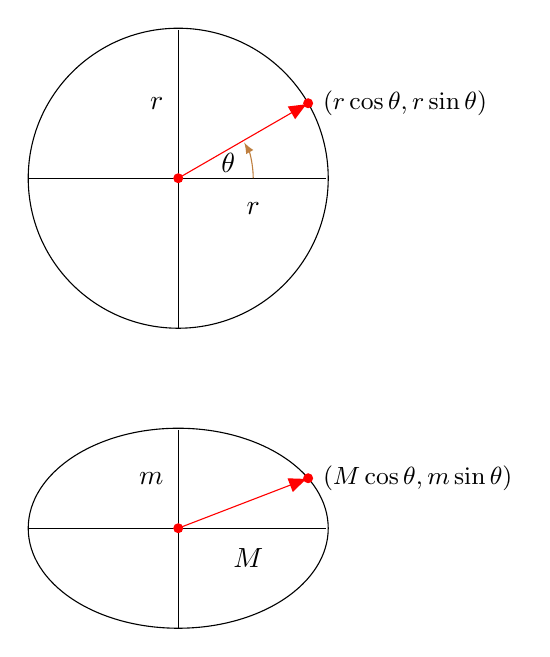
\begin{tikzpicture}[x=0.25in,y=0.25in]
\begin{scope}[>=triangle 45,shorten >=0.01in]

    \draw[black] (-3.0,0) -- (3.0,0);
    \draw[black] (0,-3.0) -- (0,3.0);
    \fill[red] (0,0.0) circle(0.1);
    \draw[black] (-0.1,1.5) node[left]{$r$};
    \draw[black] (1.5,-0.6) node{$r$};

    \draw[black] (0,0) circle(3.0);
    \fill[red] (2.598076,1.5) circle(0.1);
    \draw[red,->] (0,0) -- (2.598076,1.5);
    \draw[black] (2.7,1.5) node[right]{\small$(r\cos\theta,r\sin\theta)$};

    \draw[brown,>=latex,->] (1.5,0) arc(0:30:1.5);
    \draw[black] (1.0,+0.3) node{$\theta$};

    \draw[black] (-3.0,-7.0) -- (3.0,-7.0);
    \draw[black] (0,-9.0) -- (0,-5.0);
    \fill[red] (0,-7.0) circle(0.1);
    \draw[black] (0,-7.0) ellipse(3.0 and 2.0);
    \draw[black] (-0.1,-6.0) node[left]{$m$};
    \draw[black] (1.4,-7.6) node{$M$};

    \fill[red] (2.598076,-6.0) circle(0.1);
    \draw[red,->] (0,-7.0) -- (2.598076,-6.0);
    \draw[black] (2.7,-6.0) node[right]{\small$(M\cos\theta,m\sin\theta)$};

\end{scope}
\end{tikzpicture}
\end{wrapfigure}
Lets call a circle with center $(0,0)$ a \key{reference circle}.
Then an arbitrary circle is made by translating the reference circle
so its center is moved to an arbitrary point. \\
~ \\
Lets call an ellipse with center $(0,0)$ and major axis aligned with
the X-axis a \key{reference ellipse}.
Then an arbitrary ellipse is made by first rotating the reference ellipse
to align its major axis in an arbitrary direction, and then
translating it so its center is moved to an arbitrary point. \\
~ \\
Conversly, if you have an arbitrary ellipse, a translation followed
by a rotation will turn it into a reference ellipse.  So we are only
going to consider reference ellipses in this section.
\end{minipage}

\medskip

The reference circle with unit radius is closely related to
the reference ellipse by the linear transformation: \\
\centerline{$L = [M*u_x,m*u_y]: (x,y) \longmapsto (M*x,m*y)$} \\
This is because: \\
\centerline{$L*(\cos\theta,\sin\theta) = (M*\cos\theta,m*\sin\theta)$}

More explicitly, let $S$ be any set of points in ${\mathcal R}^2$
and define $L * S = \{ L*p: p \in S \}$.
Let $C$ be the reference circle of radius 1, which we will
call the \key{reference unit circle}, and let $E$ be the reference
ellipse with major axis $M$ and minor axis $m$.

Then $L*C = E$.

This is important because of the following.

First, note that $L^{-1}$, the inverse of $L$, exists (because
$M,m>0$) and is such that \\
\centerline{$L^{-1} = (M^{-1}*u_x,m^{-1}*u_y): (x,y)
            \longmapsto (M^{-1}*x,m^{-1}*y)$} \\
\centerline{$L^{-1}*(M*\cos\theta,m*\sin\theta) = (\cos\theta,\sin\theta)$} \\
so $L^{-1}*E=C$.

Then
\begin{itemize}
\item If $S$ is a straight line tangent to $C$, then $L*S$ is a straight
line tangent to $E$.
\item If $S$ is a straight line tangent to $E$, then $L^{-1}*S$ is a straight
line tangent to $C$.
\end{itemize}

In general, for any linear transformation $K$ and straight line
$S$, $K*S$ is a straight line.  This is because for some point
$p$ and vector $v$, \\
\hspace*{0.5in}\begin{tabular}{ll}
$S$ & $= \{ p+s*v : s~\mathrm{is~a~scalar}\}$ \\
$K*S$
    & $= \{ K*(p+s*v) : s~\mathrm{is~a~scalar}\}$ \\
    & $= \{ K*p+s*(K*v) : s~\mathrm{is~a~scalar}\}$ \\
\end{tabular} \\
That is, linear transformations like $L$ `preserve' straight lines.

Also, if $K$ is a 1-1 map (as both $L$ and $L^{-1}$ are),
and if $S_1$ and $S_2$ are two sets of points, then
$K*(S_1\cap S_2) = (K*S_1)\cap(K*S_2)$.
That is, intersections are `preserved'.  A straight line is tangent
to an ellipse or circle if and only if the two intersect in a single
point, and as intersections and straight lines are preserved, tangency
is preserved by $L$ and $L^{-1}$.

Now consider the problem of finding the point $t$ on the reference ellipse
where a straight line passing through a point $p$ external to the
ellipse and tangent to the ellipse touches the ellipse.  Then
$T=L^{-1}*t$ is the point on $C$ where a straight line passing through
the point $P=L^{-1}*p$ and tangent to $C$ touches $C$.  Using the
methods of page~\pageref{FINDING-TANGENT-POINT} we can find $T$ and
therefore $t=L*T$.

Now consider the problem of finding the point $q$ on the reference ellipse
that is closest to $p$.
The key fact is that the tangent to the ellipse at $q$ must be perpendicular
to the line $pq$.  If it were not, sliding $q$ along the ellipse in one
direction would decrease $||q-p||$.

Lets restate the problem slightly.  Let \\
\centerline{$q_\theta = (M*\cos\theta,m*\sin\theta)$} \\
and find $\theta$ such that $||q_\theta - p||$ is minimal.
Note that as $\theta$ increases, $q_\theta$ moves counter-clockwise
around the ellipse.

The tangent to the ellipse at $q_\theta$ has direction \\
\centerline{$\mathrm{azm}~dq_\theta/d\theta =
             \mathrm{azm}~(-M*\sin\theta,m*\cos\theta)$} \\
which is pointed in the counter-clockwise direction around the
ellipse.  Notice that this is an increasing function of $\theta$.

The direction of $pq_\theta$ is \\
\centerline{$\mathrm{azm}~(q_\theta-p) =
             \mathrm{azm}~(M*\cos\theta - p_x,
	                   m*\sin\theta - p_y)$} \\
and we will consider the difference \\
\centerline{$D(\theta) = \mathrm{azm}~dq_\theta/d\theta
                       - \mathrm{azm}~(q_\theta-p)$}
with the goal of finding $\theta$ such that $D(\theta) = -90~\mathrm{degrees}$,
the point where rotating the direction of $pq_\theta$ by 90 degrees clockwise
will give the counter-clockwise direction of the tangent.

\begin{minipage}{\textwidth}\raggedright
\label{INTERSECTION-PICTURE}
\begin{wrapfigure}{r}{0.42\textwidth}
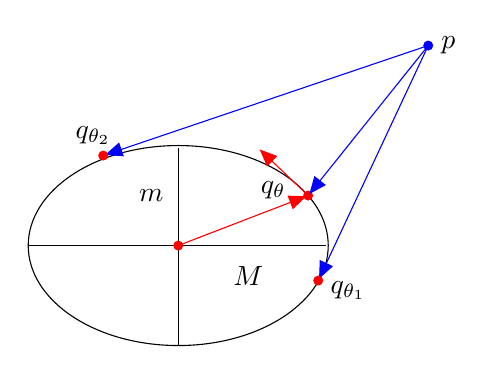
\begin{tikzpicture}[x=0.25in,y=0.25in]
\begin{scope}[>=triangle 45,shorten >=0.01in]

    \fill[blue] (5.0,0.0) circle(0.1)
              + (0.4,0.0) node[black]{$p$};

    \draw[black] (-3.0,-4.0) -- (3.0,-4.0);
    \draw[black] (0,-6.0) -- (0,-2.0);
    \fill[red] (0,-4.0) circle(0.1);
    \draw[black] (0,-4.0) ellipse(3.0 and 2.0);
    \draw[black] (-0.1,-3.0) node[left]{$m$};
    \draw[black] (1.4,-4.6) node{$M$};

    \fill[red] (2.598076,-3.0) circle(0.1);
    \draw[red,->] (0,-4.0) -- (2.598076,-3.0);
    \draw[black] (1.9,-2.9) node{$q_\theta$};
    \draw[red,->] (2.598076,-3.0) -- (1.6,-2.05);

    \draw[blue,->] (5.0,0.0) -- (2.598076,-3.0);
    \draw[blue,->] (5.0,0.0) -- (2.8,-4.7);
    \fill[red] (2.8,-4.7) circle(0.1)
             + (+0.6,-0.2) node[black]{$q_{\theta_1}$};
    \draw[blue,->] (5.0,0.0) -- (-1.5,-2.2);
    \fill[red] (-1.5,-2.2) circle(0.1)
             + (-0.2,+0.4) node[black]{$q_{\theta_2}$};
\end{scope}
\end{tikzpicture}
\end{wrapfigure}
Using methods above, we can find two angles $\theta_1<\theta_2$
such that the lines $pq_{\theta_1}$ and $pq_{\theta_2}$
are tangent to the ellipse.  See picture.

\smallskip

\begin{tabular}{@{}ll}
Then	& $D(\theta) = \mathrm{azm}~dq_\theta/d\theta
		     - \mathrm{azm}~(q_\theta-p)$ \\
and	& $\mathrm{azm}~dq_\theta/d\theta$ is \\
        & an increasing function of $\theta$ \\
and	& $\mathrm{azm}~(q_\theta-p)$ is a \\
        & decreasing function of
          $\theta \in [\theta_1,\theta_2]$ \\
so	& $D(\theta)$ is an increasing function \\
        & of $\theta \in [\theta_1,\theta_2]$ \\
and	& $D(\theta_1) = -180$ \\
and	& $D(\theta_2) = -0$ \\
so	& $D(\theta) = -90$ for some
          $\theta \in [\theta_1,\theta_2]$ \\
\end{tabular}
\end{minipage}

Therefore we can use binary search to find
$\theta \in [\theta_1,\theta_2]$ such that
$D(\theta) = -90$, making $q_\theta$ the closest
point on the ellipse to $p$.

\begin{minipage}{\textwidth}\raggedright
\label{INTERSECTION-PICTURE}
\begin{wrapfigure}{r}{0.5\textwidth}
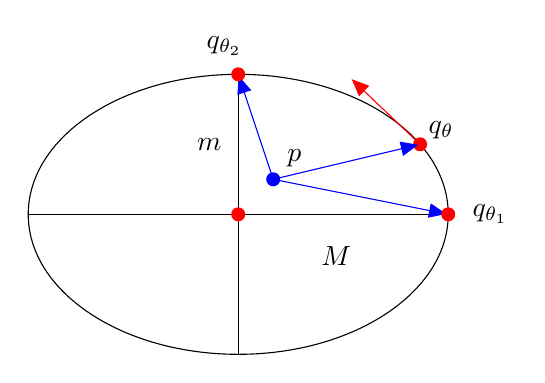
\begin{tikzpicture}[x=0.35in,y=0.35in]
\begin{scope}[>=triangle 45,shorten >=0.01in]

    \fill[blue] (0.5,0.5) circle(0.1)
              + (+0.3,+0.3) node[black]{$p$};

    \draw[black] (-3.0,0) -- (3.0,0);
    \draw[black] (0,-2.0) -- (0,+2.0);
    \fill[red] (0,0) circle(0.1);
    \draw[black] (0,0) ellipse(3.0 and 2.0);
    \draw[black] (-0.1,+1.0) node[left]{$m$};
    \draw[black] (1.4,-0.6) node{$M$};

    \fill[red] (2.598076,1.0) circle(0.1)
             + (0.3,0.2) node[black]{$q_\theta$};
    \draw[red,->] (2.598076,1.0) -- (1.6,1.95);

    \draw[blue,->] (0.5,0.5) -- (2.598076,1.0);
    \draw[blue,->] (0.5,0.5) -- (3,0);
    \fill[red] (3,0) circle(0.1)
             + (+0.6,0) node[black]{$q_{\theta_1}$};
    \draw[blue,->] (0.5,0.5) -- (0,2);
    \fill[red] (0,2) circle(0.1)
             + (-0.2,+0.4) node[black]{$q_{\theta_2}$};
\end{scope}
\end{tikzpicture}
\end{wrapfigure}
The situation when $p$ is inside the ellipse is
both similar and different.  In this case we set
$\theta_1$ and $\theta_2$ according to which
quadrant $p$ is in.  Assume $p$ is in the first
quadrant: see picture.  Then we set $\theta_1=0$ and
$\theta_2=90$.

\smallskip

\begin{tabular}{@{}ll}
Then	& $D(\theta) \begin{array}[t]{cl}
                     = & \mathrm{azm}~dq_\theta/d\theta \\
		     - & \mathrm{azm}~(q_\theta-p) \\
		     \end{array}$ \\
and	& $\mathrm{azm}~dq_\theta/d\theta$ is \\
        & an increasing function of $\theta$ \\
and	& $\mathrm{azm}~(q_\theta-p)$ is a \\
        & increasing function of
          $\theta \in [\theta_1,\theta_2]$ \\
so	& $D(\theta)$ may both increase and decrease \\
        & for $\theta \in [\theta_1,\theta_2]$ \\
and	& $D(\theta_1) > 90$ \\
and	& $D(\theta_2) < 90$ \\
so	& $D(\theta) = 90$ for some
          $\theta \in (\theta_1,\theta_2)$ \\
\end{tabular}
\end{minipage}

Again we can use binary search to find
$\theta \in [\theta_1,\theta_2]$ such that
$D(\theta) = 90$, but this time, because $D(\theta)$ is not
monotone for $\theta \in [\theta_1,\theta_2]$, we cannot
be sure that $q_\theta$ is the closest
point on the ellipse to $p$.  Specifically,
$D(\theta) = 90$ might be true for more than one
$\theta \in [\theta_1,\theta_2]$, in which case one of the
$q_\theta$ would be a point on the ellipse farthest from
$p$ for small changes in $\theta$.

We can invoke any of the following arguments to assure
ourselves that this cannot happen.

\begin{enumerate}
\item Our `geometric intuition'.
\item Graphing $D(\theta)$ in particular cases to see what
actually happens in these cases.
\item Proving that $d^2 D(\theta)/d\theta^2 > 0$ for
$\theta \in [\theta_1,\theta_2]$, thus proving the $D(\theta)$
is convex on $[\theta_1,\theta_2]$ and verifying that the graphs
are not just typical, but are general.  This is too difficult
so we will not do it.
\end{enumerate}

TBD

\end{document}
